%!TEX root = ../thesis_main.tex
%!TEX encoding = UTF-8 Unicode

%%%%%%%%%%%%%%%%%%%%%%%%%%%%%%%%%%%%%%%%%%%%%%%%%%%%%%%%%%%%%%%%%%%%
%%                                                                %%
%%                          PREAMBLE                              %%
%%                                                                %%
%%%%%%%%%%%%%%%%%%%%%%%%%%%%%%%%%%%%%%%%%%%%%%%%%%%%%%%%%%%%%%%%%%%%

%\documentclass[a4paper,twoside,10pt,draft]{memoir} %Compilation rapide
\documentclass[a4paper,twoside,10pt,final]{memoir} %Compilation lente

%!TEX encoding = UTF-8 Unicode
%!TEX root = ../thesis_main.tex


%%%%%%%%%%%%%%%%%%%%%%%%%%%%%%%%%%%%%%%%%%%%%%%%%%%%%%%%%%%%%%%%%%%%
%%                                                                %%
%%                        AUTHOR AND TITLE                        %%
%%                                                                %%
%%%%%%%%%%%%%%%%%%%%%%%%%%%%%%%%%%%%%%%%%%%%%%%%%%%%%%%%%%%%%%%%%%%%

\newcommand{\mytitle}{Robust optimisation of the pathway\texorpdfstring{\\ towards a sustainable whole-energy system}{}}
\newcommand{\mysubtitle}{A hierarchical multi-objective\texorpdfstring{\\ Reinforcement Learning-based approach}{}}
\newcommand{\myauthor}{Xavier Rixhon}

\def\eg{e.g.,\ }
\def\ie{i.e.,\ }
\def\og{``}
\def\fg{''}
\def\deg{$^{circ}$}


\usepackage[record,style=alttreegroup,nomain,symbols]{glossaries-extra}
\glsdisablehyper
%!TEX encoding = UTF-8 Unicode
%!TEX root = ../thesis_main.tex

%%%%%%%%%%%%%%%%%%%%%%%%%%%%%%
%	MATH SYMBOLS							%
%%%%%%%%%%%%%%%%%%%%%%%%%%%%%%

\glsxtrsetgrouptitle{Abreviation}{Abreviation}
\glsxtrsetgrouptitle{Notation}{Notation}

% \newcommand{\sdot}{{\bullet}}
\newcommand{\sdot}{(\cdot)}

% ---------------------------------------------------------------------------- %
% ACRONYMS
%% A

%% P
\newabbreviation[group={Acronyms}]{PCE}{PCE}{Polynomial Chaos Expansion}

%% S
\newabbreviation[group={Acronyms}]{SDGs}{SDGs}{Sustainable Development Goals}

%% U
\newabbreviation[group={Acronyms}]{UQ}{UQ}{Uncertainty Quantification}

% ---------------------------------------------------------------------------- %
% ROMAN
%% A
%\glsxtrnewsymbol[group={rs},description={ith ambient particle}]{ai}{\ensuremath{A_i}}


% ---------------------------------------------------------------------------- %
% GREEK
%\glsxtrnewsymbol[group={gs},description={Yaw angle [$\deg$]}]{beta}{\ensuremath{\beta}}


% ---------------------------------------------------------------------------- %
% Sub- Superscripts
%% A
%\glsxtrnewsymbol[group={ss},description={Relative to the ambient}]{uA}{\ensuremath{\sdot_{A}}}



\renewcommand\glstreegroupheaderfmt[1]{\begingroup\textbf{#1}\vspace{-.2cm}\par\endgroup}
\glsfindwidesttoplevelname
\glsxtrsetgrouptitle{Acronyms}{Acronyms}
\glsxtrsetgrouptitle{rs}{Roman Symbols}
\glsxtrsetgrouptitle{gs}{Greek Symbols}
\glsxtrsetgrouptitle{ss}{Sub- Superscripts}
\glsxtrsetgrouptitle{o}{Operators}

%------------------------
%% A
%\newcommand{\ABL}[2]{$U_\mABL=\SIms{#1}$ - $TI_\mABL={#2}\%$}
%------------------------
%% B

%------------------------
%% C

%------------------------
%% D
\newcommand{\degree}{^\circ}
\newcommand{\dd}{\mathrm{d}}

%------------------------
%% E
\newcommand{\etal}{\textit{et~al.}}
\newcommand{\eg}{e.g.\ }

%------------------------
%% F

%------------------------
%% G

%------------------------
%% H

%------------------------
%% I
\newcommand{\ie}{i.e.\ }

%------------------------
%% K

%------------------------
%% L

%------------------------
%% M

%------------------------
%% N

%------------------------
%% O

%------------------------
%% P

%------------------------
%% Q

%------------------------
%% R

%------------------------
%% S

%------------------------
%% T


%------------------------
%% U
\newcommand{\uh}{\hat{u}}
\newcommand{\uv}{\mathbf{u}} 

\newcommand{\ub}{\boldsymbol{u}} 

\newcommand{\uconvw}{\tilde{U}_W}

%------------------------
%% V
\newcommand{\vv}{\mathbf{v}}
\newcommand{\vb}{\boldsymbol{v}}

%------------------------
%% W
\newcommand{\wv}{\mathbf{w}}
\newcommand{\wb}{\boldsymbol{w}}
\newcommand{\WT}{{\scriptscriptstyle \mathrm{WT}}}

%------------------------
%% X
\newcommand{\xv}{\mathbf{x}}
\newcommand{\xb}{\boldsymbol{x}}

%------------------------
%% Y
\newcommand{\yv}{\mathbf{y}}
\newcommand{\yb}{\boldsymbol{y}}

%------------------------
%% Z
\newcommand{\zv}{\mathbf{z}}
\newcommand{\zb}{\boldsymbol{z}}

%%%%%%%%%%%%%%%%%%%%%%%%%%%%%%
%	OPERATORS 								%
%%%%%%%%%%%%%%%%%%%%%%%%%%%%%%
\newcommand{\der}[2]{\frac{d #1}{d #2}}
\newcommand{\pder}[2]{\frac{\partial #1}{\partial #2}}
\newcommand{\pdern}[3]{\frac{\partial^#3 #1}{\partial #2^#3}}

\newcommand{\avgt}[1]{\left\langle {#1}\right\rangle}
\newcommand{\avgs}[1]{\overline{#1}}

%%%%%%%%%%%%%%%%%%%%%%%%%%%%%%
%	REFERENCES 							%
%%%%%%%%%%%%%%%%%%%%%%%%%%%%%%

\newcommand{\eqqref}[1]{Eq.~\eqref{#1}}
\newcommand{\seqqref}[1]{Eqs.~\eqref{#1}}
\newcommand{\eqqrefs}[2]{Eqs.~\eqref{#1} and \eqref{#2}}
\newcommand{\eqqrefc}[2]{Eqs.~\eqref{#1}, \eqref{#2}}
\newcommand{\eq}[1]{Eq.~\eqref{#1}}
% \newcommand{\eqs}[1]{Eqs.~(\ref{#1})}

\newcommand{\fig}{Fig.~\ref}
\newcommand{\figs}{Figs.~\ref}
\newcommand{\tab}{Table~\ref}
\newcommand{\sect}{Section~\ref}
\newcommand{\chap}{Chapter~\ref}
\newcommand{\chaps}{Chapters~\ref}
\newcommand{\app}{Appendix~\ref}
\newcommand{\apps}{Appendices~\ref}

%%%%%%%%%%%%%%%%%%%%%%%%%%%%%%
%	CAPTIONS							%
%%%%%%%%%%%%%%%%%%%%%%%%%%%%%%
% Color palette
  
\usepackage{xcolor}
\definecolor{myBlue}{rgb}{0.25, 0.25, 0.75}
\definecolor{myRed}{rgb}{0.8, 0.1, 0.3}
\definecolor{myGrey0}{rgb}{0.25, 0.25, 0.25}
\definecolor{myGrey1}{rgb}{0.50, 0.50, 0.50}
\definecolor{myGrey2}{rgb}{0.75, 0.75, 0.75}


\definecolor{Blue0}{rgb}{0.7752402921953095, 0.8583006535947711, 0.9368242983467897}
\definecolor{Blue1}{rgb}{0.41708573625528644, 0.6806305267204922, 0.8382314494425221}
\definecolor{Blue2}{rgb}{0.1271049596309112, 0.4401845444059977, 0.7074971164936563}
\definecolor{Blue3}{rgb}{0.03137254901960784, 0.18823529411764706, 0.4196078431372549}

\definecolor{BluePy}{rgb}{0.69140625, 0.8164, 0.8868}
\definecolor{RedC}{rgb}{0.9453, 0.7266, 0.6602}

\definecolor{gw}{rgb}{1, 0, 0}
\definecolor{jb}{rgb}{0, 1, 0}
\definecolor{tg}{rgb}{0, 0, 1}
\definecolor{jh}{rgb}{1, 1, 0}

\newcommand{\gw}[1]{{#1}}
% \newcoxmmand{\gw}[1]{\textcolor{gw}{#1}}
\newcommand{\jb}[1]{\textcolor{jb}{#1}}
\newcommand{\tg}[1]{\textcolor{tg}{#1}}
\newcommand{\jh}[1]{\textcolor{jh}{#1}}


%%%%%%%%%%%%%%%%%%%%%%%%%%%%%%%%%%%%%%%%%%%%%%%%%%%%%%%%%%%%%%%%%%%%
%%                                                                %%
%%                       LANGUAGE AND FONTS                       %%
%%                                                                %%
%%%%%%%%%%%%%%%%%%%%%%%%%%%%%%%%%%%%%%%%%%%%%%%%%%%%%%%%%%%%%%%%%%%%

% -- Language ------------------------------------------------------
\usepackage[utf8]{inputenc}
\usepackage[USenglish]{babel}
\usepackage[T1]{fontenc} % Accents
\usepackage{scrextend} % to use \footref: multiple reference to the same table footnote
\usepackage{pbox} % to have new line inside table cells

% -- Fonts ---------------------------------------------------------
%\usepackage{lmodern}
%% utopia
%\usepackage{fourier}
%% palatino
%\usepackage{palatino}
%% pifont
%\usepackage{pifont}
%% charter
%\usepackage{charter}

% stix
\usepackage[lcgreekalpha]{stix}
\usepackage{textcomp}

%% better and newer palatino font
%\usepackage{newpxtext,newpxmath}

%% special font, no ams package included...
%\usepackage[full]{textcomp}
%\usepackage[osf]{newtxtext} % osf for text, not math
%\usepackage{cabin} % sans serif
%\usepackage[varqu,varl]{inconsolata} % sans serif typewriter
%\usepackage[bigdelims,vvarbb]{newtxmath} % bb from STIX
%\usepackage[cal=boondoxo]{mathalfa} % mathcal


%%%%%%%%%%%%%%%%%%%%%%%%%%%%%%%%%%%%%%%%%%%%%%%%%%%%%%%%%%%%%%%%%%%%
%%                                                                %%
%%                    TEXT, LAYOUT AND STRUCTURE                  %%
%%                                                                %%
%%%%%%%%%%%%%%%%%%%%%%%%%%%%%%%%%%%%%%%%%%%%%%%%%%%%%%%%%%%%%%%%%%%%

% -- Paragraphs---- ------------------------------------------------
\linespread{1.15}
%\usepackage[parfill]{parskip} %% NOT working with memoir class... see https://tex.stackexchange.com/questions/193485/how-to-use-usepackageparfillparskip-in-memoir-class for discussion

% -- Margins -------------------------------------------------------
\usepackage[includehead,includefoot,centering,height=20cm,width=12cm,showframe=false]{geometry}
%\usepackage[includehead,includefoot,centering,height=20cm,width=12cm,showframe=false]{geometry}

%\usepackage[includehead,includefoot,centering,height=20cm,width=12cm,showframe=true]{geometry} %taille des marges
%\usepackage[includehead, includefoot, top=4.2cm, bottom=5.4cm, left=4.5cm, right=4.5cm,showframe=true]{geometry}%…PhP
%\usepackage[includehead, includefoot, top=4.8cm, bottom=4.8cm, left=4.5cm, right=4.5cm,showframe=true]{geometry}%4.8 4.8

% -- Layout --------------------------------------------------------
%\usepackage{layout} % pour afficher le layout des pages

%\usepackage{color}
%\usepackage[dvipsnames]{xcolor}s
\usepackage{lineno}
%\usepackage{ulem} %underline for emphasis
\usepackage{fancyhdr}% pour en-tetes personnalises
\usepackage{appendix} % gestion appendix
\usepackage{tikz}% pour diagrammes
\usetikzlibrary{shapes.misc}
\usepackage{setspace}

%\usepackage{titlepages} % for the titlepage examples

%\usepackage{charter}
%\usepackage[raggedright]{titlesec} % evite les coupures de mot dans les titres

\usepackage{afterpage} % Force content to be on the next page

%% The lineno packages adds line numbers. Start line numbering with
%% \begin{linenumbers}, end it with \end{linenumbers}. Or switch it on
%% for the whole article with \linenumbers.
\usepackage{lineno} % Line numbers

\sloppy % evite les debordements de texte dans la marge
\raggedbottom %regroupe les espaces verticaux automatiques au bas des pages

% -- Structure et Paragraphes --------------------------------------
%evite les lignes veuves et orphelines
\clubpenalty=10000
\widowpenalty=10000
\interfootnotelinepenalty=10000

%\setcounter{secnumdepth}{3} % numerote les subsubsections
\setsecnumdepth{subsection}
\maxtocdepth{subsection}

% -- Style ---------------------------------------------------------
\normalfont
% chapter style
%\chapterstyle{ell}
%\chapterstyle{madsen}
%\chapterstyle{bianchi}
%\chapterstyle{dash}
%\chapterstyle{thatcher}
\newcommand{\clearemptydoublepage}{\newpage{\pagestyle{empty}\cleardoublepage}} %pour effacer les en-tetes sur la page vierge avant chaque chapitre

%\pagestyle{ruled}
\nouppercaseheads
\pagestyle{headings}
\makeheadrule{headings}{\textwidth}{0.3pt}


%%%%%%%%%%%%%%%%%%%%%%%%%%%%%%%%%%%%%%%%%%%%%%%%%%%%%%%%%%%%%%%%%%%%
%%                                                                %%
%%                     TABLES AND FIGURES                         %%
%%                                                                %%
%%%%%%%%%%%%%%%%%%%%%%%%%%%%%%%%%%%%%%%%%%%%%%%%%%%%%%%%%%%%%%%%%%%%

% -- Figures -------------------------------------------------------
\usepackage{graphicx}
\graphicspath{{frontend/img/}{chap_intro_ccl/img/}{chap_case_study/img/}{chap_ES_PCE/img/}{chap_electro_uq/img/}{chap_methodo/img/}{chap_myopic/img/}{chap_RL/img/}{chap_atom_mol/img/}{chap_RobPol/img/}{appendices/img/}} % Figures folder different for each input
%\graphicspath{{img/}} %
\DeclareGraphicsExtensions{.eps,.pdf,.png,.jpg}

%\usepackage[cleanup,process=auto]{pstool}
%\usepackage[cleanup,process=all]{pstool} % force process every figure
%\usepackage{pst-pdf}
%\usepackage{epstopdf}
%\usepackage{auto-pst-pdf} 
%\usepackage{psfrag}
%\PassOptionsToPackage{psfrag}{process=none}

\usepackage[figuresright]{rotating} %https://tex.stackexchange.com/questions/337/how-to-change-certain-pages-into-landscape-portrait-mode

\def\figwidth{0.9\textwidth}
\newcommand{\singlefigwidth}{.75\textwidth}

\setfloatadjustment{figure}{\centering}
\setfloatlocations{figure}{thb}
\newsubfloat{figure}

\newcommand{\illusname}{Illustration}
\newcommand{\listillusname}{List of Illustrations}
\newlistof{listofillus}{loillu}{\listdiagramname}
\newfloat[chapter]{illustration}{loillu}{\illusname}
\newlistentry{illustration}{loillu}{0}
\renewcommand\theillustration{\arabic{illustration}}    

\usetikzlibrary{shapes}

% -- Tables --------------------------------------------------------
\usepackage{booktabs} % Table customization: \specialrule

\usepackage{longtable} % Long tables on multiple pages
\usepackage{tabu}
\usepackage{ltablex} % Use ltablex instead of tabularx
\usepackage{multirow} % Cellule de tableau sur plusieurs lignes
\usepackage{multicol} % Cellule de tableau sur plusieurs colonnes
\usepackage{dcolumn} % Columns aligned on decimal point
\newcolumntype{d}[1]{D{.}{.}{#1}}
\usepackage{array} % ??

%\usepackage{cellspace} % Espace entre le texte et les bord des cellules
%\usepackage{tabularx} % Tableau avec largeur fixée

\usepackage{makecell} % Customize table headers with \thead
\renewcommand\theadfont{\bfseries} % Customize table column headers with \thead

% -- Sub-figures and Captions --------------------------------------
\usepackage{subfig}
\usepackage{wrapfig} % Images dans le texte
%\usepackage{floatrow} % Tableau et figure côte à côte
%\usepackage{subcaption} % sub caption

\usepackage[labelfont=bf, labelsep=period, justification=justified,singlelinecheck=false]{caption} % style et taille de police des captions
%\captionsetup[table]{position=below}

%\captionnamefont{\sffamily} % font for the "Figure xx" part
%\captionnamefont{\footnotesize\sffamily} % font for the "Figure xx" part
%\captionnamefont{\footnotesize} % font for the "Figure xx" part
%\captiontitlefont{\footnotesize} % font for the caption part
%\captiontitlefont{\small}
% change caption witdth
%\changecaptionwidth
%\captionwidth{0.9\textwidth}
%\captionstyle[\centering]{}


%%%%%%%%%%%%%%%%%%%%%%%%%%%%%%%%%%%%%%%%%%%%%%%%%%%%%%%%%%%%%%%%%%%%
%%                                                                %%
%%                      SCIENTIFIC PACKAGES                       %%
%%                                                                %%
%%%%%%%%%%%%%%%%%%%%%%%%%%%%%%%%%%%%%%%%%%%%%%%%%%%%%%%%%%%%%%%%%%%%

% -- Math ----------------------------------------------------------
\usepackage{amsmath}
%\usepackage[intlimits]{amsmath}
\usepackage{amsfonts}
\usepackage{amsthm} % Extended theorem environments
%\usepackage{amssymb} % Math symbols %%redundant with stix package
%\usepackage{esint} % Intégrales multiples
%\usepackage{esvect} % Vecteurs
\usepackage{mathtools}
\usepackage{pifont}

% Put the equation label in the document, to help writing
\usepackage{showlabels}
%\usepackage[final]{showlabels} %disable

\usepackage[boxed]{algorithm2e}

% -- Physics and Chemistry -----------------------------------------
\usepackage{siunitx} % SI units
\usepackage[version=4]{mhchem} % Chemical equations

% -- Symbols -------------------------------------------------------
\usepackage[super]{nth} %text superscript \nth{i}
\usepackage{textcomp} % Degree symbol °, and certainly others
%\newcommand{\cmark}{\ding{51}}
%\newcommand{\xmark}{\ding{55}}


%%%%%%%%%%%%%%%%%%%%%%%%%%%%%%%%%%%%%%%%%%%%%%%%%%%%%%%%%%%%%%%%%%%%
%%                                                                %%
%%                  BIBLIOGRAPHY AND HYPERREF                     %%
%%                                                                %%
%%%%%%%%%%%%%%%%%%%%%%%%%%%%%%%%%%%%%%%%%%%%%%%%%%%%%%%%%%%%%%%%%%%%

% -- Bibliography --------------------------------------------------
% For natbib help, see http://merkel.texture.rocks/Latex/natbib.php?lang=fr
%\usepackage{biblatex}
\usepackage[square,numbers,sort&compress]{natbib}
%\setlength{\bibsep}{0.5pt}
%\usepackage{pdfcomment}
%\usepackage[square,numbers,compress]{natbibtooltip}
\usepackage{textcomp} % recognize the textquotesingle from bib

\bibliographystyle{options/elsarticle-num-names}  %Ordered by appearance in the text, with DOI and URL

%\bibliographystyle{options/elsarticle-num}  %Same but \citet command does not work
%\bibliographystyle{options/elsarticle-harv}  %Harvard style (Author, year, no number)
%\bibliographystyle{options/elsarticle-num-names-nourldoi}  %Ordered by appearance in the text, with DOI
%\bibliographystyle{options/elsarticle-names-nourldoi}  %Ordered by alphabet, with DOI
%\bibliographystyle{options/elsarticle-names-nourl} %Ordered by alphabet, without DOI
%\bibliographystyle{options/model4-names}

% -- Hyperref ------------------------------------------------------
\PassOptionsToPackage{hyphens}{url} %this helps breaking URL when too long
\usepackage[bookmarks,hidelinks]{hyperref}
\usepackage{cleveref}
\usepackage{bm} % To use \bm in order to get bold math symbols

% PDF metadata
\hypersetup{pdftitle={\mytitle}}
\hypersetup{pdfauthor={\myauthor}}
\hypersetup{pdfsubject={PhD thesis}}
\hypersetup{pdfkeywords={Energy System Modelling,EnergyScope,Reinforcement Learning,Policy Optimisation, Electro-fuels}}

% Links color
\newcommand\myshade{85}
% from http://latexcolor.com
\definecolor{airforceblue}{rgb}{0.36, 0.54, 0.66}
\definecolor{battleshipgrey}{rgb}{0.52, 0.52, 0.51}
\definecolor{burntumber}{rgb}{0.54, 0.2, 0.14}
\definecolor{sangria}{rgb}{0.57, 0.0, 0.04}
\colorlet{mylinkcolor}{sangria}
\colorlet{mycitecolor}{battleshipgrey}

%\hypersetup{
%%linkcolor  = mylinkcolor!\myshade!black,
%%citecolor  = mycitecolor!\myshade!black,
%%urlcolor   = myurlcolor!\myshade!black,
%colorlinks = true,
%}

%\hypersetup{
%    colorlinks=true,
%    citecolor = blue,
%    linkcolor=blue,
%    urlcolor = blue
% }

%% Links with color frame
\hypersetup{
colorlinks = false,
%citebordercolor ={red},
}

%% No color on links (for printing)
%\hypersetup{hidelinks}

% Adding bookmarks to pdf (works after clearing aux and then 2 clean compilations)
%\hypersetup{bookmarks={true}} % --> does it by default

%% Reference with Fancy Tooltips (only works with the dedicated compilation script)
%from: https://tex.stackexchange.com/questions/84681/interactive-pdf-latex-and-article-of-the-future/84700#84700
%\usepackage[inactive,blur=0.6, fixcolor]{fancytooltips}
%\usepackage[inactive]{fancytooltips}

% -- Footnotes ------------------------------------------------------
\newcommand\blfootnote[1]{%
  \begingroup
  \renewcommand\thefootnote{}\footnote{#1}%
  \addtocounter{footnote}{-1}%
  \endgroup} %%Footnotes sans numéro

%%!TEX encoding = UTF-8 Unicode
%!TEX root = ../thesis_main.tex

%%%%%%%%%%%%%%%%%%%%%%%%%%%%%%
%	MATH SYMBOLS							%
%%%%%%%%%%%%%%%%%%%%%%%%%%%%%%

\glsxtrsetgrouptitle{Abreviation}{Abreviation}
\glsxtrsetgrouptitle{Notation}{Notation}

% \newcommand{\sdot}{{\bullet}}
\newcommand{\sdot}{(\cdot)}

% ---------------------------------------------------------------------------- %
% ACRONYMS
%% A

%% P
\newabbreviation[group={Acronyms}]{PCE}{PCE}{Polynomial Chaos Expansion}

%% S
\newabbreviation[group={Acronyms}]{SDGs}{SDGs}{Sustainable Development Goals}

%% U
\newabbreviation[group={Acronyms}]{UQ}{UQ}{Uncertainty Quantification}

% ---------------------------------------------------------------------------- %
% ROMAN
%% A
%\glsxtrnewsymbol[group={rs},description={ith ambient particle}]{ai}{\ensuremath{A_i}}


% ---------------------------------------------------------------------------- %
% GREEK
%\glsxtrnewsymbol[group={gs},description={Yaw angle [$\deg$]}]{beta}{\ensuremath{\beta}}


% ---------------------------------------------------------------------------- %
% Sub- Superscripts
%% A
%\glsxtrnewsymbol[group={ss},description={Relative to the ambient}]{uA}{\ensuremath{\sdot_{A}}}



\renewcommand\glstreegroupheaderfmt[1]{\begingroup\textbf{#1}\vspace{-.2cm}\par\endgroup}
\glsfindwidesttoplevelname
\glsxtrsetgrouptitle{Acronyms}{Acronyms}
\glsxtrsetgrouptitle{rs}{Roman Symbols}
\glsxtrsetgrouptitle{gs}{Greek Symbols}
\glsxtrsetgrouptitle{ss}{Sub- Superscripts}
\glsxtrsetgrouptitle{o}{Operators}

%------------------------
%% A
%\newcommand{\ABL}[2]{$U_\mABL=\SIms{#1}$ - $TI_\mABL={#2}\%$}
%------------------------
%% B

%------------------------
%% C

%------------------------
%% D
\newcommand{\degree}{^\circ}
\newcommand{\dd}{\mathrm{d}}

%------------------------
%% E
\newcommand{\etal}{\textit{et~al.}}
\newcommand{\eg}{e.g.\ }

%------------------------
%% F

%------------------------
%% G

%------------------------
%% H

%------------------------
%% I
\newcommand{\ie}{i.e.\ }

%------------------------
%% K

%------------------------
%% L

%------------------------
%% M

%------------------------
%% N

%------------------------
%% O

%------------------------
%% P

%------------------------
%% Q

%------------------------
%% R

%------------------------
%% S

%------------------------
%% T


%------------------------
%% U
\newcommand{\uh}{\hat{u}}
\newcommand{\uv}{\mathbf{u}} 

\newcommand{\ub}{\boldsymbol{u}} 

\newcommand{\uconvw}{\tilde{U}_W}

%------------------------
%% V
\newcommand{\vv}{\mathbf{v}}
\newcommand{\vb}{\boldsymbol{v}}

%------------------------
%% W
\newcommand{\wv}{\mathbf{w}}
\newcommand{\wb}{\boldsymbol{w}}
\newcommand{\WT}{{\scriptscriptstyle \mathrm{WT}}}

%------------------------
%% X
\newcommand{\xv}{\mathbf{x}}
\newcommand{\xb}{\boldsymbol{x}}

%------------------------
%% Y
\newcommand{\yv}{\mathbf{y}}
\newcommand{\yb}{\boldsymbol{y}}

%------------------------
%% Z
\newcommand{\zv}{\mathbf{z}}
\newcommand{\zb}{\boldsymbol{z}}

%%%%%%%%%%%%%%%%%%%%%%%%%%%%%%
%	OPERATORS 								%
%%%%%%%%%%%%%%%%%%%%%%%%%%%%%%
\newcommand{\der}[2]{\frac{d #1}{d #2}}
\newcommand{\pder}[2]{\frac{\partial #1}{\partial #2}}
\newcommand{\pdern}[3]{\frac{\partial^#3 #1}{\partial #2^#3}}

\newcommand{\avgt}[1]{\left\langle {#1}\right\rangle}
\newcommand{\avgs}[1]{\overline{#1}}

%%%%%%%%%%%%%%%%%%%%%%%%%%%%%%
%	REFERENCES 							%
%%%%%%%%%%%%%%%%%%%%%%%%%%%%%%

\newcommand{\eqqref}[1]{Eq.~\eqref{#1}}
\newcommand{\seqqref}[1]{Eqs.~\eqref{#1}}
\newcommand{\eqqrefs}[2]{Eqs.~\eqref{#1} and \eqref{#2}}
\newcommand{\eqqrefc}[2]{Eqs.~\eqref{#1}, \eqref{#2}}
\newcommand{\eq}[1]{Eq.~\eqref{#1}}
% \newcommand{\eqs}[1]{Eqs.~(\ref{#1})}

\newcommand{\fig}{Fig.~\ref}
\newcommand{\figs}{Figs.~\ref}
\newcommand{\tab}{Table~\ref}
\newcommand{\sect}{Section~\ref}
\newcommand{\chap}{Chapter~\ref}
\newcommand{\chaps}{Chapters~\ref}
\newcommand{\app}{Appendix~\ref}
\newcommand{\apps}{Appendices~\ref}

%%%%%%%%%%%%%%%%%%%%%%%%%%%%%%
%	CAPTIONS							%
%%%%%%%%%%%%%%%%%%%%%%%%%%%%%%
% Color palette
  
\usepackage{xcolor}
\definecolor{myBlue}{rgb}{0.25, 0.25, 0.75}
\definecolor{myRed}{rgb}{0.8, 0.1, 0.3}
\definecolor{myGrey0}{rgb}{0.25, 0.25, 0.25}
\definecolor{myGrey1}{rgb}{0.50, 0.50, 0.50}
\definecolor{myGrey2}{rgb}{0.75, 0.75, 0.75}


\definecolor{Blue0}{rgb}{0.7752402921953095, 0.8583006535947711, 0.9368242983467897}
\definecolor{Blue1}{rgb}{0.41708573625528644, 0.6806305267204922, 0.8382314494425221}
\definecolor{Blue2}{rgb}{0.1271049596309112, 0.4401845444059977, 0.7074971164936563}
\definecolor{Blue3}{rgb}{0.03137254901960784, 0.18823529411764706, 0.4196078431372549}

\definecolor{BluePy}{rgb}{0.69140625, 0.8164, 0.8868}
\definecolor{RedC}{rgb}{0.9453, 0.7266, 0.6602}

\definecolor{gw}{rgb}{1, 0, 0}
\definecolor{jb}{rgb}{0, 1, 0}
\definecolor{tg}{rgb}{0, 0, 1}
\definecolor{jh}{rgb}{1, 1, 0}

\newcommand{\gw}[1]{{#1}}
% \newcoxmmand{\gw}[1]{\textcolor{gw}{#1}}
\newcommand{\jb}[1]{\textcolor{jb}{#1}}
\newcommand{\tg}[1]{\textcolor{tg}{#1}}
\newcommand{\jh}[1]{\textcolor{jh}{#1}}


\begin{document}


%%%%%%%%%%%%%%%%%%%%%%%%%%%%%%%%%%%%%%%%%%%%%%%%%%%%%%%%%%%%%%%%%%%%
%%                                                                %%
%%                       FRONT MATTER                             %%
%%                                                                %%
%%%%%%%%%%%%%%%%%%%%%%%%%%%%%%%%%%%%%%%%%%%%%%%%%%%%%%%%%%%%%%%%%%%%

%!TEX encoding = UTF-8 Unicode 
%!TEX root = ../thesis_main.tex
\begin{titlingpage}

\begin{figure}[!t]
\begin{minipage}[m]{.46\textwidth}
\flushleft

\includegraphics[width=\textwidth]{UCL_immc.pdf}
\end{minipage}
\hfill
\begin{minipage}[m]{.40\textwidth}
\flushright
\vspace{-0.25cm}

\includegraphics[width=\textwidth]{BEST_SPF.pdf}
\end{minipage}
\vspace{3 cm}
\end{figure}

\vspace{2 cm}

%\begin{flushleft}
%\rule[-0,2 cm]{\textwidth}{1mm}
%\end{flushleft}

\begin{flushright}
\vspace{0.2cm}
{\fontsize{16}{20}\selectfont \mytitle\\[1em]
{\fontsize{14}{16}\selectfont \mysubtitle}}
\end{flushright}

\begin{flushright}
%\begin{center}
\rule{0.75\linewidth}{0.2mm}
%\end{center}
\end{flushright}

\begin{flushright}
\vspace{1 cm}
\begin{small}
Doctoral dissertation presented by\\
\vspace{0.1cm}
{\Large \textbf{Xavier \textsc{Rixhon}}}\\
\vspace{0.1cm}
%Ingénieur,\\
in partial fulfillment of the requirements for\\
the degree of Doctor in Engineering Sciences\\[1em]%
\end{small}
\end{flushright}

\begin{flushright}
\begin{small}
September 2024\\%
\end{small}
%\vspace{0.5 cm}
\end{flushright}


\vspace{\fill}
%\centering
\begin{small}
%\resizebox{\linewidth}{!}{
\begin{tabular}{l}
%\toprule
%\multicolumn{1}{l}{\textbf{Composition du jury}}\\
\textbf{Thesis committee}\\
%\toprule
\selectfont
Pr. Francesco \textsc{Contino} (UCLouvain, Supervisor) \\ 
Pr. Hervé \textsc{Jeanmart} (UCLouvain, Supervisor) \\ 
Pr. Paul \textsc{Fisette} (UCLouvain, President) \\ 
Pr. Christophe \textsc{De Vleeschouwer} (UCLouvain, Secretary) \\ 
Pr. Sylvain \textsc{Quoilin} (ULiège) \\
Dr. Stefano \textsc{Moret} (ETH Zurich)\\
Pr. Stefan \textsc{Pfenninger} (TU Delft)\\

%\bottomrule
% mettre par ordre alphabétique 
\end{tabular} 
%}
\end{small}
%
\clearpage
%\thispagestyle{empty}
\vspace*{\fill}{\center{
\copyright \hspace{0.1cm} 2023\\
Xavier Rixhon\\
All Rights Reserved\\}}

\end{titlingpage}





\frontmatter

% -- Abstract ------------------------------------------------------
%!TEX root = ../thesis_main.tex
%!TEX encoding = UTF-8 Unicode

\thispagestyle{empty}

\begin{abstract}

This thesis will be awesome

\end{abstract}

\clearpage
\clearemptydoublepage

% -- Quote ---------------------------------------------------------
%!TEX root = ../thesis_main.tex
%!TEX encoding = UTF-8 Unicode

\thispagestyle{empty}

\begin{figure}[p!]
\hfill \begin{minipage}[c]{.7\textwidth}
\begin{flushright}
\textit{Be the smile 
you wish to see on the face of the world.}
\\[1em]
-- adapted from Mahatma Gandhi\\
\end{flushright}
\end{minipage}
\end{figure}

\clearpage
\clearemptydoublepage

% -- Remerciements -------------------------------------------------
\chapter*{Remerciements}
%!TEX root = ../thesis_main.tex
%!TEX encoding = UTF-8 Unicode

Thank you, thank you, far too kind
\clearemptydoublepage

% -- Contents ------------------------------------------------------
\thispagestyle{empty}
%\mbox{}
\tableofcontents*
\clearemptydoublepage

\printunsrtglossaries


%%%%%%%%%%%%%%%%%%%%%%%%%%%%%%%%%%%%%%%%%%%%%%%%%%%%%%%%%%%%%%%%%%%%
%%                                                                %%
%%                        MAIN MATTER                             %%
%%                                                                %%
%%%%%%%%%%%%%%%%%%%%%%%%%%%%%%%%%%%%%%%%%%%%%%%%%%%%%%%%%%%%%%%%%%%%

\mainmatter

% -- Introduction --------------------------------------------------
\chapter*[Introduction]{Introduction}
\addcontentsline{toc}{chapter}{Introduction}
It has been proven that the climate change, among other environmental challenges, is (mostly) due to the concentration of anthropogenic \gls{GHG} in the environment \cite{IPCC_CO2_budget}. Therefore, the \gls{GHG} emissions from human activities must be mitigated to prevent further environmental damages. Among these emissions, globally, about 75\% are directly related to the whole-energy system \cite{ourworldindata_CO2_world}. The \gls{GHG} emissions usually expressed in kt$_{\ce{CO2},\text{eq}}$, could be developed as an adapted, \ie less economy-oriented, version of the original Kaya identity \cite{kaya1997environment}:

\begin{equation}
\label{eq:equality_GHG}
\mathrm{GHG} =  \frac{\mathrm{GHG}}{\text{Primary energy}} \times \frac{\text{Primary energy}}{\mathrm{EUD}}\times \frac{\mathrm{EUD}}{\text{Population}} \times \text{Population}\\
 \end{equation}

\noindent
where the first term represents the \gls{GWP} of the primary energy mix, the second is the inverse of the efficiency and the third could stand as the energy intensity per capita. Such an identity, mathematically-correct though, is criticized for the arbitrary choice of variables, the non-independence of them usually leading to the rebound effect and its global/encompassing approach that does not translate properly the heterogeneity of the situation \cite{IPCC2000}. However, Eq. \ref{eq:equality_GHG} has the merit to highlight three levers of action that should be activated to reduce the \gls{GHG} emissions and, consequently, favour the transition, leaving aside the question of the total population and its growth \cite{dodson2020population,scovronick2017impact}. These three levers of actions are: renewables, efficiency and sufficiency aiming at reducing the first, the second and the third terms on the right-hand side of Eq. \ref{eq:equality_GHG}, respectively. The latter, explicitly mentioned by the IPCC for the first time in 2022 \cite{IPCC2022}, is defined by \citet{lage2023citizens} as ``a strategy for reducing, in absolute terms, the consumption and production of end-use products and services through changes in social practices in order to comply with environmental sustainability while ensuring an adequate social foundation for all people''. Altough this finds a growing interest in the scientific community \cite{o2018good}, it requires, maybe more than the two other levers, interdisciplinarity \cite{schmidt2015interdisciplinary}, \ie the combination of multiple academic disciplines like sociology, psychology or politics, that are out of the scope of my expertise, and, consequently, this thesis. However, the work developed in the present manuscript aims at providing support to such interdisciplinary projects to assess sufficiency policies. More within the grasp of the engineering world, this thesis rather focuses on the first two terms of Eq. \ref{eq:equality_GHG}, \ie renewables and efficiency. This aligns with the current European policies binding the Member States of the European Union. For instance, the Renewable Energy Directive (RED) III, published in October 2023 \cite{REDIII}, highlights that ``the Union’s climate neutrality objective (by 2050) requires a just energy transition which leaves no territory or citizen behind\footnote{This directly relates to sufficiency as it encompasses social justice in parallel with a minimization of the energy use.}, an increase in energy efficiency and significantly higher shares of energy from renewable sources in an integrated energy system'' (\ie 42.5\% of the Union's gross final consumption of energy by 2030). 

\section*{Context and motivations}

To ensure the energy supply of an assumably more and more demanding society in a context of environmental crisis, major transformations are needed (see Figure \ref{fig:intro:IEA_WEO_2019}). Besides behavioral changes, an overall reshape of the energy system is necessary in terms of both primary energy sources, \ie more renewables, and technologies used to convert these resources into the \gls{EUD} (\ie the energy service required by the the final consumer), \ie more efficiency \cite{iea2020world,luderer2018residual}. The former corresponds to a whole ``fuel switch'' (see Figure \ref{fig:intro:IEA_WEO_2019}) where energy carriers called, in the literature, ``\emph{biofuels}'', ``\emph{electrofuels}'', ``\emph{synthetic fuels}'', ``\emph{renewable fuels}'' or even ``\emph{sustainable fuels}'', will more and more play a crucial role. To avoid the confusion between these fuels and thereby reduce misunderstanding in political or academic discussions, we have suggested a comprehensive and harmonised taxonomy (see Appendix \ref{app:Taxonomy}). In the rest of this thesis, the electro - and bio - fuels are considered as renewable and with no \gls{GWP}.  

\begin{figure}[ht!]
\centering
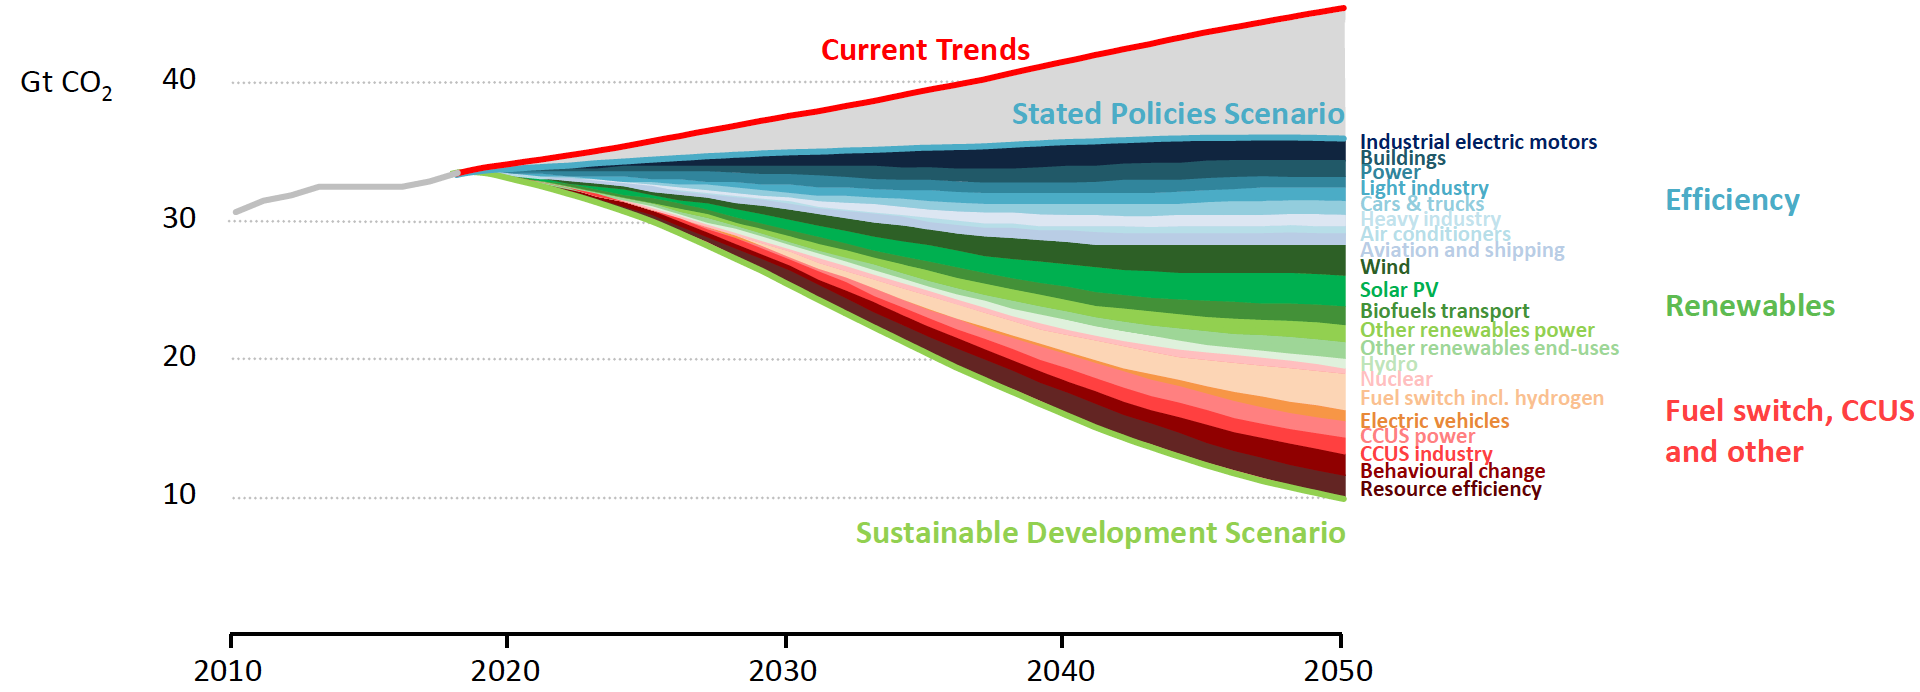
\includegraphics[width=\textwidth]{IEA_WEO_2019.png}
\caption{Energy-related CO2 emissions and reductions by sources in the Sustainable Development Scenario \cite{iea2020world}.}
\label{fig:intro:IEA_WEO_2019}
\end{figure}

In the general perspective to decrease the \gls{GWP} of the primary energy mix, \gls{VRES} like wind and solar, have already emerged as the keystone to defossilise the energy system. However, their intermittency and space disparity could hold back their vaster integration in the future. To address this issue, due to some limitations (\eg range, power, costs) of electricity-focused solutions like \gls{DC} lines, the transport and long-term storage of the renewable electricity produced in excess should be optimised. This challenge can be tackled by \textit{electrofuels} \cite{rozzi2020}. These fuels represent energy carriers where electricity has the major share in the energy balance of the fuel. In practice, this electricity is mainly converted into hydrogen (\ie electrolysis) and then potentially upgraded into more complex fuels (\eg methane, methanol or ammonia). Even if the share of electricity increases in the energy system through the electrification of the end-use demand, gaseous and liquid fuels will keep on being big players during (and after) the energy transition \cite{Ahlgren2012}. They offer three main advantages: infrastructure compatibility, storage and capacity to link sectors (\ie from electricity to mobility, heat, or industry). Development on electrofuels aims at getting them more and more compatible with existing and mature technologies \cite{Ahlgren2012}. An example is carbon-free ammonia-hydrogen blends burned in spark ignition engines \cite{lhuillier2020experimental} or \gls{CHP} applications \cite{pochet202022}. With a growing share of \gls{VRES}, sector coupling is essential to absorb the surplus of electricity from these intermittent production means \cite{robinius2017linking} and integrate them more cost-effectively \cite{brown2018response, limpensECOS2021}. Besides direct electrification of other sectors (\eg electrical heat pumps, \gls{BEV}), \citet{brown2018synergies} showed that converting power to hydrogen and methane was advantageous at high shares of renewables, in their optimisation of the European whole-energy system. Electrofuels have the ability to couple energy and non-energy sectors \cite{Stancin2020}. For instance, electricity produced in excess from \gls{VRES} can be converted into ammonia through the Haber-Bosch process and subsequently transformed into fertiliser - coupling the power and industry sectors \cite{verleysen2020can}. Gas networks present much more storage potential than electrical network (\eg 50 times more in Germany and 300 times more in France) \cite{Rosa2017}. Where batteries exhibit limited storage capacity (up to 10\,MWh) as well as self-discharge losses, electrofuels are an economical solution for high capacity (from 100 GWh) and long-term (\ie from months to years) storage of energy \cite{child2018role, dias2020energy} (see Figure \ref{fig:intro:Storage_electrofuels}). In their analysis of the German transport sector in 2050, \citet{millinger2021electrofuels} highlighted that producing electrofuels can represent a better usage of the ambient \ce{CO2} than \gls{CCS} to supply hydrocarbon fuels while limiting the curtailment of \gls{VRES}. Moreover, some applications (\eg marine, aviation and heavy-duty transport) will be hard to electrify and keep on requiring high-density energy carriers \cite{horvath2018techno, brynolf2018}. These carriers, currently produced from fossil resources, will still consist of hydrocarbons in a renewable world. This is why this thesis rather uses "defossilisation" rather than "decarbonisation" as carbon will still play a key role in a carbon-neutral energy transition \cite{mertens2020carbon}.

\begin{figure}[htbp!]
\centering
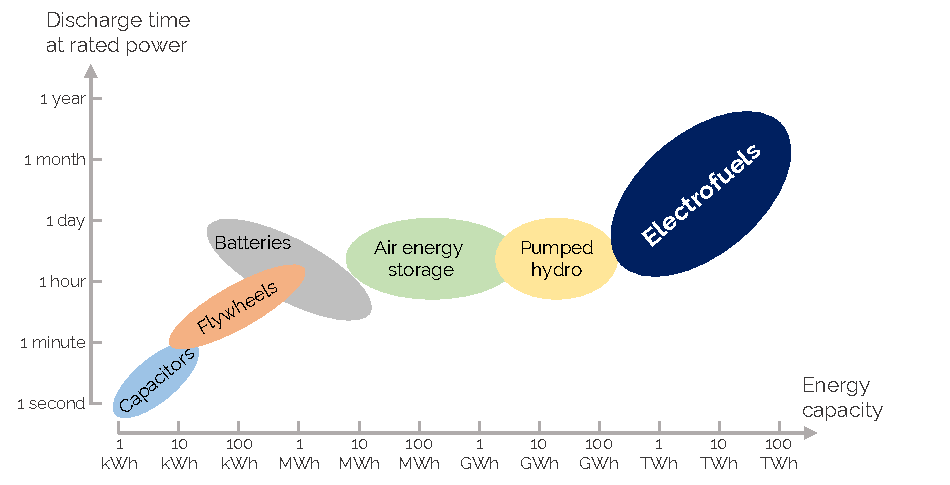
\includegraphics[width=0.9\textwidth]{Storage_electrofuels.pdf}
\caption{Energy carriers and technologies to store electricity. Electrofuels are an economical solution for high capacity and long-term storage of energy. Graph adapted from \cite{ISPT2017}.}
\label{fig:intro:Storage_electrofuels}
\end{figure}

To harvest the maximum potential of synthetic energy carriers in a sustainable transition and maximise the overall system efficiency \cite{mathiesen2015}, it is necessary to study the integration of these fuels within a multi-sector and whole-energy system \cite{Contino2020}. To reach this goal, an energy system optimisation model (ESOM) can optimise the design and the operation of the system to minimise, for instance, its costs or its emissions \cite{zeng2011review}. 

In this research field of energy system planning and scenario analysis, \citet{yue2018review} highlighted that most of ESOMs use a deterministic approach (\ie 75\% out of the 134 reviewed ESOM studies). However, the model structures are inherently uncertain as well as their numerous composing parameters, especially when it comes to define an energy transition strategy for a large-scale system, such as a country. Given the lifetime of the conversion technologies, such strategy implies decisions with long-term impacts (20 to 50 years) where forecasts can be highly unreliable \cite{Moret2017}. Besides the uncertainty on the model structure (not addressed in this work), this long-term and large-system optimisation motivates the need to account for \gls{UQ} and consider it as a major challenge of such models \cite{pfenninger2014energy}. This challenge, along with a large number (\ie more than a hundred) of uncertain parameters and limited information of their distribution, leads to the "curse of dimensionality" \cite{kuo2005lifting}, where the computational burden rapidly explodes with the number of considered uncertain parameters.

On top of dealing with these uncertainties, the reality of decision-makers is a limited foresight into the future \cite{poncelet2016myopic}. In a perfect foresight approach, decision-makers would be able to, from now on, see the ``finish-line of the transition'', \ie 2050 (and beyond), and make the planning decisions once and for all accordingly. On the contrary, they uncover the realisation of these uncertainties step-by-step (\ie in a ``myopic'' way), and progressively act on them to, hopefully, meet the set target to mitigate the climate change. In the objective to respect an overall \ce{CO2}-budget rather than to follow a prescribed \ce{CO2}-emissions trajectory, there was a need for a framework to explore these multiple transition pathways and provide insight about intermediate milestones not to miss. On top of the ``what to do?'', this approach aims at helping the policymakers to answer the  question ``how to do it?''.

Finally, when assessing the robustness of transition pathways provided by \gls{ESOMs}, the literature shows a variety of techniques, \eg Monte-Carlo analysis, stochastic programming or robust optimisation \cite{yue2018review}. However, the robustness is commonly applied to assess the sensibility of the solution regarding the objective function to optimise (\ie the total cost).  Given the complexity of whole-energy system models (\ie multiple sectors and multiple energy carriers) along with the time-scale of the transition and the lot of uncertainties, the total cost does not provide information on the sensibility of the design strategy, \ie the investment decisions. Where \citet{moret2020overcapacity} proposed a method to assess the robustness of a design by investigating the potential overcapacity needed to face uncertainties. However, their work focused on the power sector only and for a target future year, \ie 2035.  The literature was missing an approach to tackle these two challenges: to go beyond the total transition cost encompassing the details of a solution into a single value while assessing the whole-energy system over its whole transition.

\section*{Objectives and tasks}
``\textit{Our task is not to foresee the future, but to enable it.}'' Saint-Exupéry in Citadelle, 1948. In that sense, this thesis aims at providing decision-makers with new methods and informed policies accounting for the intrinsic uncertainties of the future.  Rather than trying, in vain, to answer the question ``What could possibly happen in the future?'', this work rather addresses the ``What could or should we do to make the future possible?''. Given these general context and motivations, the research questions are described as follows:
\begin{itemize}
\item What is the role of electrofuels in the transition pathway of a whole-energy system subject to uncertainties, limited foresight into the future and a \ce{CO2}-budget? What are the key uncertainties driving their import?
\item How to explore the multiple pathway possibilities through the optimisation of a policy, \ie sequence of actions to support a transition?
\item How to assess the robustness of a pathway roadmap defining the design strategy over the transition?
\end{itemize}

To answer these questions, several tasks have been carried out on the whole-energy system model accounting for the uncertainties, the method to explore the myopic pathway of such a system and the approach to assess the robustness of a pathway roadmap.  All this work has been applied to the case of Belgium, a densely populated country with a limited amount of renewable energies, which represents roughly one third of the forecast energy demand \cite{Limpens2020}. This makes it a challenging case to go from a highly fossil-dominated system in 2020 (\ie 73\% of the primary energy mix \cite{spf_economy_2022}) to carbon-neutrality by 2050. 

The model developed and used in the context of this thesis is EnergyScope Pathway \cite{limpens2024pathway}. First introduced by Limpens in his PhD thesis \cite{limpens2021generating}, this model optimises the design and the operation of a whole-energy system over several decades and accounts for the pathway transition from an existing system to a long term target, \ie 2050.  Compared to other models, EnergyScope Pathway introduces a rapid (\ie around 15~min on a personal laptop for the optimisation of a 30-year transition) computational optimisation tool for exploring diverse transition pathways within an entire energy system while maintaining temporal precision (\ie hourly time-resolution) to accurately capture the integration of \gls{VRES}. Based on this model originally implemented in a perfect foresight approach, \ie one overall optimisation for the whole pathway, we have developed the myopic method. In this, the whole time horizon (\ie 30 years) is optimised through a sequence of 10-year long time-windows having a 5-year overlap between each other. To address the question about the role of electrofuels, we have detailed further on their implementation in the model to account for four main ones: hydrogen, methane, ammonia and methanol. Moreover, given their current and (expected) future role into the sector of the \gls{NED}, we have implemented this sector with a similar level of detail as the other sectors of the system, \ie electricity, heat and transport. 

To account for uncertainties, we have used, and adapted to our case study, the work of \citet{Moret2017PhDThesis} and \citet{coppittersthesis} on the uncertainty characterisation and quantification, respecitvely. In his thesis, \citet{Moret2017PhDThesis} developed a framework to obtain uncertainty range for a variety of parameters like cost of purchasing and availability of resources or investment cost and efficiency of technologies. These ranges have then been sampled and propagated through the EnegyScope Pathway via the RHEIA framework developed by \citet{coppittersthesis}. Using the surrogate-modeling approach called \gls{PCE}, this framework allows identifying the uncertain parameters with the biggest impact on the variation of total transition cost or other outputs of interest like the imported amount of electrofuels. 

To explore the different pathway trajectories in this myopic optimisation process, we have applied the \gls{RL} method where an ``agent'' is trained through its interactions with its environment, EnergyScope Pathway, to optimise its policy, \ie sequence of actions to take to support the transition. Starting from the initial state of the energy system in 2020, the agent takes every five years a set of actions until reaching 2050. Although, these actions are taken every five years, they impact the system, for the next ten years - their time window. The intermediate solutions obtained in the middle of the time window are used as a new starting point for the agent that makes a new series of decisions for the next ten years, etc. Repeating the whole transition with different sequences of actions-states allow the agent to come up with an optimised policy towards sustainability, considering the variation of the parameters of its environment.

Finally, in the objective to assess the sensibility to uncertainties of different design transition roadmaps, we have defined an approach to come up with a ``robustness metric''. This approach is based on \gls{PCA} where directions capturing the widest design variations are identified and serve as a frame. Roadmaps resulting from perfect foresight optimisation have been tested in a myopic and uncertain pathways. The results of these myopic runs have then been ``projected'' on the aforementioned frame to be able to compare the robustness of different roadmaps between each other.

\section*{Outline}
This thesis is composed of five chapters to provide answers to the different research questions. Chapter \ref{chap:chap_methodo} brings more details about the different methodological aspects of this work. It starts with the main constraints, parameters and variables of the whole-energy system optimisation model, EnergyScope Pathway. Then, it gives information on the \gls{UQ} approach and the way it has been adapted to the case of Belgium and its transition pathway. Finally, general fundamentals and more case-specific considerations are brought up about the \gls{RL} and \gls{PCA}-based robustness approaches.

Chapter \ref{chap:case_study} presents the case study of this work, \ie Belgium and its energy transition. Without exhaustively detailing the data \cite{limpens2021generating}, this chapter focuses on the main contributions of this work regarding the case study: the \gls{NED}, the implementation of electrofuels and their respective routes of production and consumption, limiting  the cumulative emissions of the transition to a certain \ce{CO2}-budget rather than a prescribed emissions-trajectory and the date related \gls{SMR} as an option to produce nuclear-based electricity in the future.

Chapter \ref{chap:atom_mol} is the first of the three chapters presenting results. In this one, we detail the results of the \gls{GSA} carried out on the Belgian energy transition under the lens of the atom-molecules dilemma. On top of the impact of uncertainties on the total transition cost and the system design in general, we target the impact of having new nuclear capacities by 2040 onward and the driving parameters on the import of electrofuels.

In Chapter \ref{chap:chap_RL}, the rules of the ``\gls{RL} game'' are detailed. In other words, we define the action and state spaces as well as the reward function driving the behaviour of the agent in its quest to optimise its policy. Then, we analyse the results of the learning phase before testing under uncertainties the learned policy versus more ``classic'' myopic optimisation, \ie without the support of such a policy.

After detailing the robustness metric based on the \gls{PCA} approach, Chapter \ref{chap:chap_RobPol} assesses the robustness of different roadmaps resulting of deterministic perfect foresight optimisation under certain conditions: REF, SMR and ROB. The first one, the reference case, considers nominal values for all the uncertain parameters. The SMR case is the one introduced in Chapter \ref{chap:atom_mol} where we allow the model to install \gls{SMR} from 2040 onward. Eventually, the ROB case accounts for the highest values of parameters for those having the biggest impact on the total cost of transition (\ie cost of purchasing energy carriers, industrial \gls{EUD}, interest rate and variable \gls{OPEX} of technologies).

Finally, we draw general conclusions and suggest potential perspectives for future works in terms of uses and further developments of the methodological tools.
\clearpage

% -- Chapter 1 - Presentation of EnergyScope TD & Pathway + PCE ---------------------------------
\chapter{From a whole-energy system model and an uncertainty quantification framework}
\label{chap:chap1_ES_PCE}
%!TEX root = ../thesis_main.tex
%!TEX encoding = UTF-8 Unicode
In this chapter, we introduce the two main tools, not exhaustively of course (because already presented, in Gauthier and Diederik's theses) on which I based my work: EnergyScope and RHEIA/PCE. I'd like too to talk about the case study (Belgian energy system) that will be addressed all along the manuscript but I'm afraid it'd be too many stuff in one chapter. On the other side, I would not dedicate an entire chapter to any of these three parts. What's your opinion?
\section{EnergyScope: To optimise the energy transition pathway}
\label{sec:energyscope}

\subsection{EnergyScope TD}
\label{subsec:estd}
Presentation of the capacity to model a whole-energy system,with a hourly resolution, and of the main equations of the snapshot model (similarly to what I've done in the electrofuels+UQ paper (\url{https://www.mdpi.com/1996-1073/14/13/4027}).

\subsection{EnergyScope Pathway}
\label{subsec:espathway}
From snapshot to pathway optimisation, presentation of the main equations to link the representative years, focus on the salvage value (not presented in Gauthier's thesis but well in our Pathway paper)

\section{RHEIA: To quantify the uncertainties}
\label{sec:rheia}


\subsection{Uncertainty characterisation}
\label{subsec:uncert_charac}
Presentation here of the uncertainty characterisation from S. Moret and adding some parameters specific to the pathway model (\eg $\Delta_{\text{change}}$ linked to change speed) or specific to the main case study (\eg possibility to have nuclear SMR from 2040)


\subsection{Polynomial Chaos Expansion}
\label{subsec:pce}
Similarly to what we did in the electrofuels+UQ paper (\url{https://www.mdpi.com/1996-1073/14/13/4027}), presentation of the PCE and Sobol' sequence (which is a more optimised way to explore the ranges of uncertainties, compared, for instance, to random exploration).


\subsection{Preliminary screening and selection}
\label{subsec:screening}
Similarly to what we did in the electrofuels+UQ paper (\url{https://www.mdpi.com/1996-1073/14/13/4027}), emphasise that we only consider a limited amount of uncertain parameters to keep a reasonable computation time while capturing the impact of (almost) all the uncertainties.

\section{Case study: The Belgian energy system}
\label{sec:case_study}
Similarly to what we did in the electrofuels+UQ paper (\url{https://www.mdpi.com/1996-1073/14/13/4027}),I'd present generally here the case study, much shorter than what Gauthier did in his thesis. It'd be presenting the different sets of resources, technologies and demands.

Here, I could integrate the information on the NED and how important it is to consider it as it represents 10\% worldwide (and even 20\% in Belgium) of the energy consumption, especially because it is usually a sector that is overlooked in whole-energy system optimisation.










\clearpage


% -- Chapter 2 - UQ on a snapshot model, assessment of electrofuels ---------------------------------
\chapter{Electrofuels and uncertainties in a target future year}
\label{chap:chap2_electro_uq}
%!TEX root = ../thesis_main.tex
%!TEX encoding = UTF-8 Unicode

In this chapter aims at showing the first step of uncertainty quantification and highlight a first insight in terms of impacting parameters. It'd also highlight that depending on the gwp\_limit 
\section{From a cost-optimised to a carbon-neutral Belgian energy system: progressive defossilisation}
\label{sec:chap_2_ses_sec2}
In this section, I'd include the section 2 of the electrofuels+UQ paper (\url{https://www.mdpi.com/1996-1073/14/13/4027})(without 2.2 where I presented EnergyScope that I'd include in Chapter 1).

\subsection{Electrofuels}
\label{subsec:chap2_electrofuels}
This section would be as the section 2.1 of the electrofuels+UQ paper (\url{https://www.mdpi.com/1996-1073/14/13/4027}), where I present more specficially how electrofuels are implemented in the model

\subsection{Reference Case Study: The Belgian Energy System in 2050}
\label{subsec:chap2_case_study}
Basically section 2.3 of the electrofuels+UQ paper (\url{https://www.mdpi.com/1996-1073/14/13/4027}), where I present more specficially how electrofuels are implemented in the model where I present what a cost-optimised (without gwp-constraint) Belgian energy system would look like

\subsection{A step by step defossilisation of the snapshot system}
\label{subsec:chap2_defossilisation}
As in section 2.4, quickly show how we implement the defossilisation without having an entire pathway.

\section{Results}
\label{sec:chap2_results}
Similar to Section 4 of the electrofuels+UQ paper (\url{https://www.mdpi.com/1996-1073/14/13/4027}). There'll be work to generate up-to-date results as the model evolved (no more FC\_cars but BEV, for instance)
\subsection{Statistical analysis of the cost}
\label{subsec:chap_2_stat_analysis}

\subsection{Critical parameters}
\label{subsec:chap_2_crit_param}

\section{Discussion and perspective with the literature}
Similar to section 5.1 of the electrofuels+UQ paper (\url{https://www.mdpi.com/1996-1073/14/13/4027})

\clearpage

%% -- Chapter 3 - Myopic implementation on the pathway optimisation -----------------------------
\clearemptydoublepage
\chapter{From a perfect foresight to a myopic optimisation of the pathway} 
\label{chap:chap3_myopic}
%!TEX root = ../thesis_main.tex
%!TEX encoding = UTF-8 Unicode
In this chapter, I highlight the advantages of the myopic pathway, the methodological adaptations needed to have a myopic optimisation from EnergyScope Pathway perfect foresight and detail the difference with the perfect foresight for the case study. 

\section{Why and how myopic}
\label{sec:chap3_why_how}
Besides the fact that it is a necessary framework for the application of RL,  explain here why it is interesting, as is, to consider myopic optimisation (time saving, more appropriate to mimic policymakers' shortsightedness, etc.)

Detail the little tweeks to go from a perfect foresight to a myopic optimisation, in terms of implementation.

\section{Case study and results: Belgian energy system under \ce{CO2} trajectory}
\label{sec:chap3_case_study_results}

\subsection{Case study}
{\color{red}Question to HJ and FC : J'hésite sur le cas de référence pour la comparaison en termes de trajectoire \ce{CO2}. Voici ce à quoi je pense:
\begin{enumerate}
\item Comme ce qu'on a présenté dans le papier Pathway, une décroissance linéaire entre les émissions de 2020 et la neutralité carbone en 2050
\item Sur base du budget \ce{CO2} identique à celui de la décroissance linéaire (~1.9Gt\ce{CO2}), imposer au myopique la trajectoire \ce{CO2} issue de l'optimisation perfect foresight. Dans cette option, il y a deux sous-choix:
\begin{itemize}
\item Imposer la neutralité carbone en 2050, comme dans le cas 1.
\item Ne pas imposer la neutralité carbone en 2050
\end{itemize}
\item Sur base du budget \ce{CO2} que je donne implicitement comme objectif à mon agent (~1.2Gt\ce{CO2}), imposer au myopique la trajectoire \ce{CO2} issue de l'optimisation perfect foresight. Dans cette option, il y a deux sous-choix:
\begin{itemize}
\item Imposer la neutralité carbone en 2050, comme dans le cas 1.
\item Ne pas imposer la neutralité carbone en 2050
\end{itemize}
\end{enumerate}
Perso, je choisirais de me rapprocher le plus possible de ce que je fais ensuite avec l'agent. Du coup, ce serait le cas 3  sans imposer la neutralité carbone 2050. Dans ce cas, pour l'avoir observé, le modèle n'atteint pas la neutralité carbone. 

Quel est votre avis sur la question?
}

Define the case study and the \ce{CO2} trajectory. 

\subsection{Results and comparison with Perfect foresight}

\subsection{Discussion and perspective with the literature} 
\clearpage


%% -- Chapter 4 - Reinforcement Learning -
\clearemptydoublepage
\chapter{Reinforcement Learning \ce{CO2}-policy robust optimisation}
\label{chap:chap4_RL}
%!TEX root = ../thesis_main.tex
%!TEX encoding = UTF-8 Unicode

\section{Reinforcement learning fundamentals}
\label{sec:RL_fundamentals}
As RL is framework that is not really applied to the optimisation of the whole-energy system transition, I find it necessary to introduce the general concepts of reinforcement learning and say that, even if it is usually used in other fields, there is a point to use it here.

\section{Definition of the actions, states and rewards}
\label{sec:act_states_rew}
After pointing out that the environment is basically the EnergyScope myopic model at the different steps of the transition, define the actions, the states as well as the shape of the reward.

\subsection{Actions}
\subsection{States}
\subsection{Reward}

\section{Uncertainties in the learning}
Remind here that uncertainties considered in the learning of the agent are those presented in Chapter \ref{chap:chap1_ES_PCE} and already applied and screened in the work/results presented in Chapter \ref{chap:chap2_electro_uq}. Present as well how we affect the value of the parameters based on the value of the sample.

\section{Results}

\subsection{Training}
Here present results RL-oriented (actions, states, reward)

Then, present results energy system-oriented (installed capacities, costs, generation)

\subsection{Testing}
See how the different policies saved successively during the training behave when facing to new samples. This way, we can pick an optimal policy (the one giving the maximum average (or another metric) reward). 

We then compare the results of RL with the perfect foresight-TD deterministic and the perfect foresight-monthly with uncertainties (by setting the actions of the agent as variables in these two optimisations). The comparison would go over different aspects:
\begin{itemize}
\item Over-cost
\item Over-change, a bit like what Paolo defined as design error/change (in terms in consumed resources, installed capacities,...)
\end{itemize}



\clearpage

% -- Conclusion ----------------------------------------------------
\clearemptydoublepage
\chapter*[Conclusions]{Conclusions} 
\addcontentsline{toc}{chapter}{Conclusions}
%!TEX root = ../thesis_main.tex
%!TEX encoding = UTF-8 Unicode
I took here the same sections as in Gauthier's thesis
\section*{Thesis contributions}
\addcontentsline{toc}{section}{Thesis contributions}
Insist here on the methodological added value of the thesis

\section*{Limitations}
\addcontentsline{toc}{section}{Limitations}
\begin{itemize}
\item Due to the formulation of the salvage value, some technologies remain in place whereas they are not used anymore (see Appendix B.3, e.g. coal boilers and naphtha-cracker). It's better for the system to keep unused assets to recover part of their salvage value than prematurely decommissioning them.
\end{itemize}

\section*{Application outcomes}
\addcontentsline{toc}{section}{Application outcomes}
What this new methodology has brought over when applied to the case of Belgium

\section*{Recommendations and guidance}
\addcontentsline{toc}{section}{Recommendations and guidance}
What to do then for policymakers, how to use the tool

\section*{Perspectives}
\addcontentsline{toc}{section}{Perspectives}
List the future works to build upon the thesis

\begin{itemize}
\item \textbf{Word about sufficiency} oui mais c'est sans doute celle qui est le plus enviable car la moins risqué à tenter d'atteindre, les solutions mirages technologiques, si on y croit trop on met tout la dessus et si ca foire, on est encore plus dans la merde pcq la direction est mauvaise, la solution sobriété, meme si jamais atteint les efforts pr l'atteindre ne seront pas contre productif
\item \textbf{Word about availability of electrfuels} Voir mémoire Ced et Simon
\item Extract a roadmap representative of a multiple-run UQ or RL process.
\item In this work, we only consider emissions related to the use of energy carriers and not the construction
\end{itemize}


Quand je parle de ce que j'ai fait avec RL : Starting from the initial state of the energy system in 2020, the agent takes every five years a set of actions until reaching 2050. Although, these actions are taken every five years, they impact the system, for the next ten years --- their time window. The intermediate solutions obtained in the middle of the time window are used as a new starting point for the agent that makes a new series of decisions for the next ten years, etc. Repeating the whole transition with different sequences of actions-states allow the agent to come up with an optimised policy towards sustainability, considering the variation of the parameters of its environment.

\clearpage

%\clearemptydoublepage

%%%%%%%%%%%%%%%%%%%%%%%%%%%%%%%%%%%%%%%%%%%%%%%%%%%%%%%%%%%%%%%%%%%%
%%                                                                %%
%%                        BIBLIOGRAPHY                            %%
%%                                                                %%
%%%%%%%%%%%%%%%%%%%%%%%%%%%%%%%%%%%%%%%%%%%%%%%%%%%%%%%%%%%%%%%%%%%%

%\backmatter

%\addcontentsline{toc}{chapter}{Bibliography}
\bibliography{/Users/xrixhon/Development/GitKraken/THESIS/bib_thesis.bib}

%\clearemptydoublepage


%%%%%%%%%%%%%%%%%%%%%%%%%%%%%%%%%%%%%%%%%%%%%%%%%%%%%%%%%%%%%%%%%%%%
%%                                                                %%
%%                        APPENDICES                              %%
%%                                                                %%
%%%%%%%%%%%%%%%%%%%%%%%%%%%%%%%%%%%%%%%%%%%%%%%%%%%%%%%%%%%%%%%%%%%%

%\begin{appendices}
%
%% -- Appendix 1 - Full results -------------------------------------
%\chapter{Complete results}
%\label{chap:app_results}
%\input{appendices/full_res}


%\end{appendices}


\end{document}
